\item[(a)]
\begin{equation*}
	f(x) = max(0,x)
\Rightarrow
	f(x)' = 
	\begin{cases}
	1 & \mbox{if } x > 0 \\
	0 & otherwise
	\end{cases}
\end{equation*}
For output node j at the last layer,
\begin{equation*}
	net_j =\sum_i w_{ij}x_i
\end{equation*}
\begin{equation*}
	\frac{\partial Err}{\partial w_{ij}} = 
	\frac{\partial Err}{\partial o_j}
	\frac{\partial o_j}{\partial net_j}
	\frac{\partial net_j}{\partial w_{ij}}=
	\begin{cases}
	-(t_j-o_j)\times 1 \times  x_{ij} & \mbox{if } net_j > 0 \\
	0 & otherwise
	\end{cases}
\end{equation*}
\begin{equation*}
	\mbox{ and } \delta_j = 
	\begin{cases}
	(t_j-o_j) & \mbox{if } net_j > 0 \\
	0 & otherwise
	\end{cases}
\end{equation*}
\begin{equation*}
	\Rightarrow \Delta w_{ij} = R\delta_jx_{ij}
\end{equation*}
Back propagation rule at node j:
\begin{equation*}
	x_{jk} = o_{j}= f(\sum w_{ij} x_{ij}) \mbox{, output of node j is the input of node k.}
\end{equation*}
\begin{equation*}
	\frac{\partial Err}{\partial w_{ij}} = 
	\frac{\partial Err}{\partial net_{j}}
	\frac{\partial net_{j}}{\partial w_{ij}}
	= \sum_{k \in downstream(j)}
	\frac{\partial Err}{\partial net_{k}}
	\frac{\partial net_{k}}{\partial o_{j}}
	\frac{\partial o_{j}}{\partial net_{j}}
	\frac{\partial net_{j}}{\partial w_{ij}} 
\end{equation*}
\begin{equation*}
	\Rightarrow
	\frac{\partial Err}{\partial net_{k}} = -\delta_k,\mbox{ }
	\frac{\partial net_{k}}{\partial o_{j}}= w_{jk},\mbox{ }
	\frac{\partial o_{j}}{\partial net_{j}}= 	
		\begin{cases}
			1 & \mbox{if } net_{j} > 0 \\
			0 & otherwise
		\end{cases},\mbox{ }
	\frac{\partial net_{j}}{\partial w_{ij}}=x_{ij}
\end{equation*}
\begin{equation*}
	\Rightarrow
	\frac{\partial Err}{\partial w_{ij}} = 
	\begin{cases}
			(\sum_{k \in downstream(j)}-\delta_k w_{jk}) x_{ij}& \mbox{if } net_{j} > 0 \\
			0 & otherwise 
	\end{cases},
\end{equation*}
\begin{equation*}
	 \mbox{and }\delta_j = 
	\begin{cases}
			\sum_{k \in downstream(j)}\delta_k w_{jk}  & \mbox{if } net_{j} > 0 \\
			0 & otherwise
	\end{cases}
\end{equation*}
\begin{equation*}
	\Rightarrow \Delta w_{ij} = R\delta_jx_{ij}
\end{equation*}
\clearpage

\item[(b)]
	\begin{itemize}  
	\item[i.]	
	{\tt squared\_loss\_gradient(output, label)}:\\
	Gradient should be $-(t_j-o_j)= o_j-t_j$.
	\begin{figure}[h]
  		\centering
    	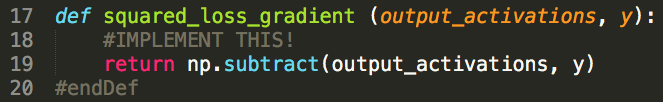
\includegraphics[width=0.7\textwidth]{fig1.png}
    	% \caption{The hidden layer h between word input and word probability output. ~\citep{rong:2014}}
	\end{figure}\\
	{\tt relu\_derivative(z)}:\\
	Relu derivative should be 
	$\begin{cases}
		1 & \mbox{if } z > 0 \\
		0 & otherwise
	\end{cases}$.
	\begin{figure}[h]
  		\centering
    	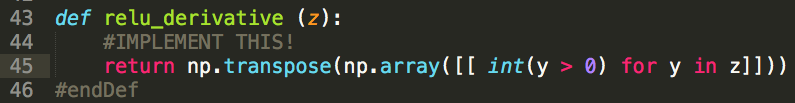
\includegraphics[width=0.7\textwidth]{fig2.png}
    	% \caption{The hidden layer h between word input and word probability output. ~\citep{rong:2014}}
	\end{figure}
	\item[ii.]
	\item[iii.]

		
	\end{itemize}